\documentclass{beamer}
\usetheme{metropolis}
\usepackage{graphicx}
\usepackage{amsmath}
\usepackage{tcolorbox}
\title{Digital Signal Processing: COSC390}
\author{Jordan Hanson}
\institute{Whittier College Department of Physics and Astronomy}

\begin{document}
\maketitle

\begin{frame}{Unit 1.3 Outline}
Previous lectures covered:
\begin{itemize}
\item Complex numbers 2: The Fourier series and Fourier transform (continuous and discrete)
\item \textit{Time-permitting}: The Laplace transform (continuous and discrete)
\end{itemize}
This lecture will cover: (Reading: \textbf{Chapter 2})
\begin{itemize}
\item \alert{Statistics and probability: the normal distribution and other useful distributions}
\item \alert{Noise: digitization and sampling}
\item Noise: Spectral properties of noise, ADC and DAC
\end{itemize}
\end{frame}

\section{Statistics and Probability: The Normal Distribution}

\begin{frame}[fragile]{Statistics and Probability: The Normal Distribution}
The \textit{mean}, $\mu$, and \textit{standard deviation}, $\sigma$, of a data set $\lbrace x_i \rbrace$ are defined as
\begin{align}
\mu &= \frac{1}{N}\sum_{i=1}^N x_i \\
\sigma^2 &= \frac{1}{N-1}\sum_{i=1}^N\left(x_i-\mu\right)^2
\end{align}
Octave commands:
\begin{verbatim}
x = randn(100,1);
mean(x)
std(x)
\end{verbatim}
\end{frame}

\begin{frame}[fragile]{Statistics and Probability: The Normal Distribution}
One nice theorem: \textit{The variance is the average of the squares minus the square of the average.}  Let $\langle x \rangle$ represent the average of the quantity or expression $x$.  We have
\begin{equation}
\sigma_x^2 = \langle x^2 \rangle - \langle x \rangle^2
\end{equation}
\end{frame}

\begin{frame}[fragile]{Statistics and Probability: The Normal Distribution}
\small
\textbf{Note}: \textit{process or signal process} versus \textit{the data}.  Just because the data has a given $\mu$ and $\sigma$ does not imply that the signal process has or will continue to have the exact same values of $\mu$ and $\sigma$.  The underlying process could be \textit{non-stationary}.
\begin{figure}
\centering
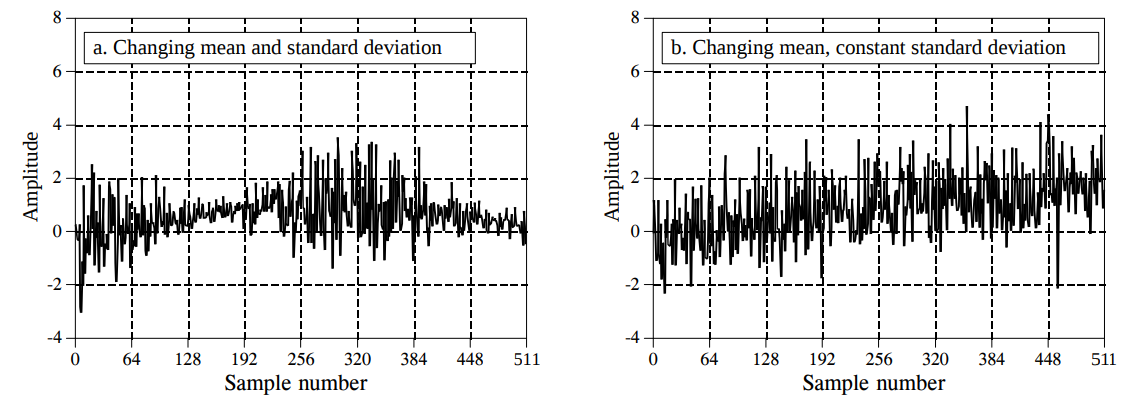
\includegraphics[width=0.9\textwidth]{figures/non_stationary.png}
\caption{\label{fig:non_stationary} Signal processes in (a) and (b) are considered \alert{non-stationary} because one or both of $\mu$ and $\sigma$ depend on time.}
\end{figure}
\end{frame}

\begin{frame}[fragile]{Statistics and Probability: The Normal Distribution}
\textbf{A histogram} is an object that represents the frequency of particular values in a signal.  For example, below is a histogram of 256,000 numbers drawn from a probability distribution:
\begin{figure}
\centering
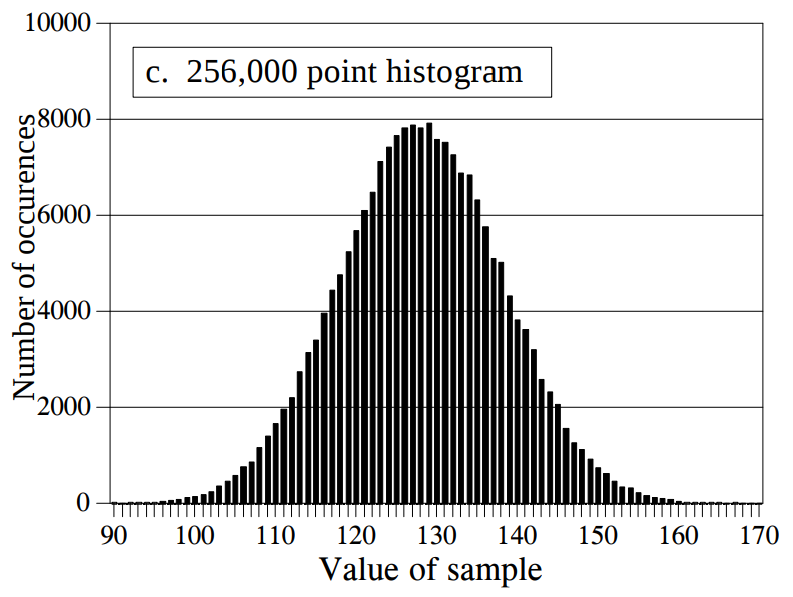
\includegraphics[width=0.55\textwidth]{figures/hist.png}
\caption{\label{fig:hist} The histogram contains counts versus sample values.}
\end{figure}
\end{frame}

\begin{frame}[fragile]{Statistics and Probability: The Normal Distribution}
The following octave code should reproduce something like Fig. \ref{fig:hist} from the textbook:
\begin{verbatim}
x = randn(256000,1)*10.0+130.0;
[b,a] = hist(x,100);
plot(a,b,'o');
\end{verbatim}
The function \textit{randn(N,M)} draws $N \times M$ numbers from a normal distribution and returns them in the size the user desires.  The function \textit{hist(x,N)} creates $N$ bins and sorts the data $x_i$ into them.
\end{frame}

\begin{frame}[fragile]{Statistics and Probability: The Normal Distribution}
\small
For data that is appropriately stationary, we can use histograms to estimate $\mu$ and $\sigma$ faster, since we only have to loop over bins rather than every data sample.  Let $H_i$ represent the counts in a given bin, and $i$ represent the bin sample.  We have:
\begin{align}
\mu &= \frac{1}{N}\sum_{i=1}^{M}i H_i \\
\sigma^{2} &= \frac{1}{N-1}\sum_{i=1}^M \left(i-\mu\right)^2 H_i
\end{align}
(To obtain the mean in signal \textit{amplitude}, you'd have to convert bin number to amplitude - more on that in a moment).
\end{frame}

\begin{frame}[fragile]{Statistics and Probability: The Normal Distribution}
\small
Some vocabulary:
\begin{itemize}
\item \textbf{normalization} - Total probability is 1.0.  For pdf - the integral from $[-\infty,\infty]$ is 1.0.  For pmf - the sum from $[-\infty,\infty]$ is 1.0.
\item \textbf{pmf} - Probability mass function: A \textit{normalized continuous function} that gives the probability of a value, given the value.
\item \textbf{histogram} - Histograms are an attempted measurement of the pmf by breaking the data into discrete bins.  Histograms can be \textit{normalized} as well.
\item \textbf{pdf} - Probability density function: A \textit{normalized continuous function} that gives the probability density of a value, given the value.  Integrating the \textit{normalized} pdf between two values gives the probability of observing data between the given values.
\end{itemize}
\end{frame}

\section{Statistics and Probability: Other Useful Distributions}

\section{Conclusion}

\begin{frame}{Unit 1.3 Outline}
Previous lectures covered:
\begin{itemize}
\item Complex numbers 2: The Fourier series and Fourier transform (continuous and discrete)
\item \textit{Time-permitting}: The Laplace transform (continuous and discrete)
\end{itemize}
This lecture will cover: (Reading: \textbf{Chapter 2})
\begin{itemize}
\item \alert{Statistics and probability: the normal distribution and other useful distributions}
\item \alert{Noise: digitization and sampling}
\item Noise: Spectral properties of noise, ADC and DAC
\end{itemize}
\end{frame}

\end{document}
